\documentclass[12pt,a4paper]{article}
\usepackage{setspace}
\usepackage{tocloft}
\usepackage{graphicx}
\usepackage{ulem}
\usepackage{titling}
\usepackage{amsmath}
\usepackage{geometry}
\usepackage{setspace}
\usepackage{ragged2e}
\usepackage{listings}
\usepackage{xcolor}
\usepackage{float}
\usepackage{fancyhdr}
\usepackage{lipsum}

\geometry{left=3.5cm, top=2.5cm, right=1.25cm, bottom=1.25cm}

\pagestyle{fancy}
\fancyhead{}
\fancyfoot{}
\fancyfoot[R]{\thepage}
\renewcommand{\headrulewidth}{0pt}
\setlength{\footskip}{20pt}
\fancypagestyle{plain}{
    \fancyhf{} % Clear all header and footer fields
    \fancyfoot[R]{\thepage} % Right-align the page number
    \renewcommand{\headrulewidth}{0pt} % Remove the header rule on chapter pages
}
\setlength{\droptitle}{-6cm}

\doublespacing

% JavaScript and MongoDB syntax highlighting
\lstdefinelanguage{JavaScript}{
    keywords={function, var, let, const, return, if, else, for, while, do, break, continue, new, try, catch, throw, finally, switch, case, default, class, extends, import, export, from, async, await},
    keywordstyle=\color{blue}\bfseries,
    ndkeywords={true, false, null, undefined, NaN, Infinity},
    ndkeywordstyle=\color{magenta}\bfseries,
    identifierstyle=\color{black},
    sensitive=false,
    comment=[l]{//},
    morecomment=[s]{/*}{*/},
    commentstyle=\color{gray}\ttfamily,
    stringstyle=\color{orange}\ttfamily,
    morestring=[b]',
    morestring=[b]"
}

\lstdefinelanguage{MongoDB}{
    keywords={use, db, find, findOne, insertOne, insertMany, updateOne, updateMany, deleteOne, deleteMany, aggregate, count, createIndex, mapReduce, ObjectId},
    keywordstyle=\color{blue}\bfseries,
    ndkeywords={true, false, null},
    ndkeywordstyle=\color{magenta}\bfseries,
    identifierstyle=\color{black},
    sensitive=false,
    comment=[l]{//},
    morecomment=[s]{/*}{*/},
    commentstyle=\color{gray}\ttfamily,
    stringstyle=\color{orange}\ttfamily,
    morestring=[b]',
    morestring=[b]"
}

% HTML syntax highlighting
\lstdefinelanguage{HTML}{
    keywords={html, head, body, title, meta, script, style, link, div, span, p, a, img, form, input, button, class, id, href, src, type, rel, alt, placeholder, method, action},
    keywordstyle=\color{blue}\bfseries,
    sensitive=false,
    comment=[s]{<!--}{-->},
    commentstyle=\color{gray}\ttfamily,
    stringstyle=\color{orange}\ttfamily,
    morestring=[b]",
    morestring=[b]'
}

% Set up the listings environment
\lstset{
    basicstyle=\ttfamily\footnotesize,
    numbers=left,
    numberstyle=\tiny\color{gray},
    stepnumber=1,
    numbersep=5pt,
    backgroundcolor=\color{white},
    frame=single,
    rulecolor=\color{black},
    breaklines=true,
    breakatwhitespace=true,
    captionpos=b,
    showstringspaces=false
}

% Title Page
\setlength{\droptitle}{-6cm}
\pagenumbering{gobble}


\title{}
\date{}
\begin{document}

\centering
\vspace{2cm}
{\large\textbf{
    MEAN: FULL STACK WEB DEVELOPMENT LABRATORY\\
    \vspace{0.5cm}
    PROJECT REPORT\\
}}
\vspace{1cm}
{
\normalsize
SUBMITTED IN PARTIAL FULFILLMENT OF THE REQUIREMENTS FOR THE AWARD OF THE DEGREE OF\\\vspace{0.8cm}
{\large \textbf{BACHELOR OF TECHNOLOGY}\\(Information Technology)}
}

\vspace{1cm}
    \begin{figure}[H]
    \centering
    
\includegraphics[width=0.475\textwidth]{assets/GNE_logo.png}
    \end{figure}
    {\large JAN-MAY, 2025}
    \vspace{1cm}

    \textbf{SUBMITTED BY:}\\
    \vspace{1cm}
    \begin{tabular}{p{8cm}p{8cm}}
    NAME: Devesh Sharma & NAME: Mayank\\
    UNIVERSITY ROLL NO: 2203818 & UNIVERSITY ROLL NO: 2203855\\
    \end{tabular}\\
    \vspace{1cm}
    {DEPARTMENT OF INFORMATION TECHNOLOGY}\\
    \vspace{0.2cm}
    {\large GURU NANAK DEV ENGINEERING COLLEGE LUDHIANA}\\
    \vspace{0.2cm}
    (An Autonomous College Under UGC ACT)

\justifying
\newpage

\begin{center}
    \textbf{ACKNOWLEDGMENT}
\end{center}
I would like to express my sincere gratitude to my project guide, Dr. Palwinder Kaur, for her invaluable guidance and support throughout this project. Her expertise in web development and MEAN stack technologies has been instrumental in shaping this work and enhancing my understanding of modern web application architecture.

I am deeply thankful to Guru Nanak Dev Engineering College for providing the necessary resources and infrastructure that made this project possible. The emphasis on practical learning and modern technologies has greatly contributed to the successful completion of this work.

Finally, I would like to thank my family and friends for their constant encouragement and support throughout my academic journey.

\newpage

\pagenumbering{arabic}
\setcounter{tocdepth}{1}
\setlength{\cftbeforesecskip}{0pt}
\setlength{\cftbeforetoctitleskip}{-1em}
\tableofcontents
\newpage

\section{Introduction}
This project implements a modern web-based AI chat application that integrates with Ollama's local Large Language Models (LLMs) while featuring user authentication and chat history persistence. The application follows the MEAN stack architecture: MongoDB for the database, Express.js for the backend server, AngularJS for the frontend interface, and Node.js as the runtime environment.

The application allows users to register, log in, create new chat sessions, and continue previous conversations with the AI. All user information and chat history are stored securely in MongoDB, providing a persistent and personalized experience. By leveraging the power of modern web technologies, this project demonstrates the practical application of full-stack development principles in creating a functional and user-friendly AI chat interface.

\section{Objectives}
\begin{itemize}
\item \textbf{To} implement a full-stack web application using the MEAN stack architecture
\item \textbf{To} integrate Ollama's local LLM capabilities for AI-powered conversations
\item \textbf{To} implement a secure user authentication system with session management
\item \textbf{To} create a persistent chat history system with MongoDB
\item \textbf{To} allow users to manage their chat sessions (create, load, update, delete)
\item \textbf{To} develop a responsive and intuitive user interface using AngularJS
\end{itemize}

\section{Technologies Used}
\begin{itemize}
\item \textbf{Database:} MongoDB for data persistence
\item \textbf{Backend:} Node.js with Express.js framework
\item \textbf{Frontend:} AngularJS for the user interface
\item \textbf{Authentication:} bcrypt for password hashing, express-session for session management
\item \textbf{AI Integration:} Ollama API for LLM interactions
\item \textbf{Additional Libraries:}
  \begin{itemize}
    \item connect-mongo for session storage
    \item axios for HTTP requests
    \item mongoose for MongoDB object modeling
  \end{itemize}
\item \textbf{Development Tools:} Visual Studio Code, Git
\end{itemize}

\section{System Architecture}
The application follows the MEAN stack architecture with four main components:
\begin{itemize}
\item \textbf{MongoDB Database:} Stores user information and chat history
\item \textbf{Express.js Backend:} Provides API endpoints for authentication, chat management, and AI interaction
\item \textbf{AngularJS Frontend:} Delivers the user interface and client-side application logic
\item \textbf{Ollama API:} External service that provides LLM capabilities
\end{itemize}

\subsection{Database Schema}
The application uses two main MongoDB collections:

\subsubsection{User Schema}
Stores user credentials and authentication information:
\begin{lstlisting}[language=JavaScript]
const UserSchema = new mongoose.Schema({
  username: {
    type: String,
    required: true,
    unique: true,
    trim: true,
  },
  password: {
    type: String,
    required: true,
  },
  createdAt: {
    type: Date,
    default: Date.now,
  }
});
\end{lstlisting}

\subsubsection{Chat Schema}
Stores chat sessions and message history:
\begin{lstlisting}[language=JavaScript]
const MessageSchema = new mongoose.Schema({
  role: {
    type: String,
    enum: ["user", "assistant"],
    required: true,
  },
  content: {
    type: String,
    required: true,
  },
  timestamp: {
    type: Date,
    default: Date.now,
  }
});

const ChatSchema = new mongoose.Schema({
  userId: {
    type: mongoose.Schema.Types.ObjectId,
    ref: "User",
    required: true,
  },
  title: {
    type: String,
    default: function() {
      return "Chat " + this.createdAt.toLocaleDateString();
    }
  },
  messages: [MessageSchema],
  createdAt: {
    type: Date,
    default: Date.now,
  },
  updatedAt: {
    type: Date,
    default: Date.now,
  }
});
\end{lstlisting}

\section{Implementation Details}

\subsection{Authentication System}
The application implements a secure authentication system using bcrypt for password hashing and express-session for session management.

\subsubsection{User Registration}
The registration endpoint handles new user creation with password hashing:
\begin{lstlisting}[language=JavaScript]
router.post("/register", async (req, res) => {
  try {
    const { username, password } = req.body;

    // Check if user exists & hash password
    const existingUser = await User.findOne({ username });
    if (existingUser) {
      return res.status(400).json({ error: "Username already exists" });
    }

    const hashedPassword = await bcrypt.hash(password, 10);

    // Create user & start session
    const user = new User({ username, password: hashedPassword });
    await user.save();
    req.session.userId = user._id;

    res.json({ success: true, username: user.username });
  } catch (err) {
    res.status(500).json({ error: "Registration failed" });
  }
});
\end{lstlisting}

\subsubsection{User Login}
The login endpoint authenticates users and establishes sessions:
\begin{lstlisting}[language=JavaScript]
router.post("/login", async (req, res) => {
  try {
    const { username, password } = req.body;

    // Find user & verify password
    const user = await User.findOne({ username });
    if (!user) return res.status(400).json({ error: "Invalid credentials" });

    const isMatch = await bcrypt.compare(password, user.password);
    if (!isMatch) return res.status(400).json({ error: "Invalid credentials" });

    // Set session and return user info
    req.session.userId = user._id;
    res.json({ success: true, username: user.username });
  } catch (err) {
    res.status(500).json({ error: "Login failed" });
  }
});
\end{lstlisting}

\subsection{Chat Management System}
The application provides complete CRUD operations for chat management:

\subsubsection{Creating a New Chat}
This endpoint allows authenticated users to create new chat sessions:
\begin{lstlisting}[language=JavaScript]
router.post("/", isAuthenticated, async (req, res) => {
  try {
    const { title, messages } = req.body;
    const chat = new Chat({
      userId: req.session.userId,
      title: title || undefined,
      messages: messages || []
    });
    await chat.save();
    res.json(chat);
  } catch (err) {
    res.status(500).json({ error: "Failed to create chat" });
  }
});
\end{lstlisting}

\subsubsection{Loading Existing Chats}
This endpoint retrieves a list of a user's previous chat sessions:
\begin{lstlisting}[language=JavaScript]
router.get("/", isAuthenticated, async (req, res) => {
  try {
    // Find user's chats, select minimal fields, sort by recent first
    const chats = await Chat.find({ userId: req.session.userId })
      .select("_id title updatedAt")
      .sort({ updatedAt: -1 });
    res.json(chats);
  } catch (err) {
    res.status(500).json({ error: "Failed to get chats" });
  }
});
\end{lstlisting}

\subsection{Integration with Ollama API}
The application integrates with Ollama's API to generate responses from the LLM and automatically saves responses to the user's chat history:

\begin{lstlisting}[language=JavaScript]
app.post("/api/chat", async (req, res) => {
  try {
    // Send user messages to Ollama API
    const response = await axios.post("http://localhost:11434/api/chat", {
      model: "llama3.2:3b",
      messages: req.body.messages,
      stream: false,
    });

    // Format AI response
    const aiMessage = {
      role: "assistant",
      content: response.data.message?.content || response.data.response,
    };

    // Save to chat history if user is authenticated
    if (req.session.userId && req.body.chatId) {
      const Chat = require("./models/Chat");
      const chat = await Chat.findOne({
        _id: req.body.chatId,
        userId: req.session.userId
      });

      if (chat) {
        chat.messages.push(aiMessage);
        chat.updatedAt = Date.now();
        await chat.save();
      }
    }

    res.json({ message: aiMessage });
  } catch (err) {
    console.error(err);
    res.status(500).json({ error: "Error connecting to Ollama" });
  }
});
\end{lstlisting}

\section{Features}
\begin{itemize}
\item \textbf{User Authentication:} Secure registration and login system
\item \textbf{Session Management:} Persistent user sessions with MongoDB storage
\item \textbf{Chat Creation:} Ability to start new chat conversations
\item \textbf{Chat History:} Saving and loading previous conversations
\item \textbf{Chat Management:} Updating chat titles and deleting unwanted chats
\item \textbf{AI Integration:} Seamless interaction with Ollama's LLM
\item \textbf{Responsive UI:} User-friendly interface with AngularJS
\end{itemize}

\section{Key Components}

\subsection{Frontend Interface}
The application features a responsive and intuitive user interface built with AngularJS that adapts based on authentication state:

\begin{lstlisting}[language=HTML]
<!-- Main application container with conditional views -->
<div class="app-container">
    <!-- Header with user info when logged in -->
    <div class="header">
        <h1>Ollama Chat</h1>
        <div class="user-info" ng-if="chat.user">
            <span>Welcome, {{chat.user.username}}!</span>
            <button ng-click="chat.logout()">Logout</button>
        </div>
    </div>

    <!-- Authentication section shown when not logged in -->
    <div class="auth-container" ng-if="!chat.user">
        <div class="auth-tabs">
            <div class="auth-tab" ng-class="{'active': chat.authTab === 'login'}">Login</div>
            <div class="auth-tab" ng-class="{'active': chat.authTab === 'register'}">Register</div>
        </div>
        <!-- Login/Register forms would be here -->
    </div>

    <!-- Main chat interface shown when logged in -->
    <div class="main-content" ng-if="chat.user">
        <!-- Sidebar with chat history -->
        <div class="sidebar">
            <button ng-click="chat.newChat()">New Chat</button>
            <ul class="chat-list">
                <li ng-repeat="chatItem in chat.chatList"
                    ng-click="chat.loadChat(chatItem._id)">
                    {{chatItem.title}}
                </li>
            </ul>
        </div>

        <!-- Chat area with messages -->
        <div class="chat-container">
            <!-- Message display and input would be here -->
        </div>
    </div>
</div>
\end{lstlisting}

\subsection{AngularJS Controller}
The application's frontend logic is managed by an AngularJS controller that handles authentication, chat loading, and message sending:

\begin{lstlisting}[language=JavaScript]
angular.module("chatApp", []).controller("ChatController", function ($http) {
  var vm = this;

  // State variables
  vm.messages = [];
  vm.input = "";
  vm.loading = false;
  vm.user = null;
  vm.authTab = 'login';
  vm.chatList = [];
  vm.currentChat = null;

  // Core functionality
  vm.sendMessage = function() {
    if (!vm.input.trim()) return;

    // Add user message to display
    var userMsg = { role: "user", content: vm.input.trim() };
    vm.messages.push(userMsg);
    vm.input = "";
    vm.loading = true;

    // Send to API with current chat ID if available
    var reqData = { messages: vm.messages };
    if (vm.currentChat) reqData.chatId = vm.currentChat._id;

    $http.post("/api/chat", reqData)
      .then(function(response) {
        vm.messages.push(response.data.message);
        // Save updated chat if needed
        if (vm.currentChat) vm.updateChatTitle();
      })
      .finally(function() { vm.loading = false; });
  };

  // Initialize by checking auth status
  vm.checkAuthStatus();
});
\end{lstlisting}

\section{Deployment Process}
The source code is available on GitHub at https://github.com/mayank0304/mean-mini-project.

\begin{enumerate}
\item Install Node.js and MongoDB on the target system
\item Clone the repository containing the application code
\item Install dependencies:
   \begin{verbatim}
   npm install
   \end{verbatim}
\item Ensure MongoDB is running:
   \begin{verbatim}
   mongod --dbpath=/path/to/data/directory
   \end{verbatim}
\item Install and start Ollama service with the required model:
   \begin{verbatim}
   ollama run llama3.2:3b
   \end{verbatim}
\item Start the application:
   \begin{verbatim}
   node server.js
   \end{verbatim}
\item Access the application at http://localhost:3000
\end{enumerate}

\section{Challenges and Solutions}
\begin{itemize}
\item \textbf{Challenge:} Integrating MongoDB with Express for session storage
\item \textbf{Solution:} Used connect-mongo package to seamlessly store sessions in MongoDB

\item \textbf{Challenge:} Implementing secure authentication
\item \textbf{Solution:} Utilized bcrypt for password hashing and express-session for session management

\item \textbf{Challenge:} Managing real-time chat updates
\item \textbf{Solution:} Implemented efficient state management in AngularJS controller to maintain chat state

\item \textbf{Challenge:} Synchronizing chat history between database and frontend
\item \textbf{Solution:} Developed a robust API to handle create, read, update, and delete operations for chat sessions

\item \textbf{Challenge:} Handling asynchronous API calls to Ollama
\item \textbf{Solution:} Used async/await with proper error handling to ensure reliable communication
\end{itemize}

\section{Future Enhancements}
\begin{itemize}
\item \textbf{User Profile Management:} Allow users to update their profile information and preferences
\item \textbf{Multiple AI Model Selection:} Enable users to choose from different Ollama models
\item \textbf{Chat Categories and Tags:} Implement a system to categorize and tag chat sessions
\item \textbf{Advanced Authentication:} Add features like password reset, email verification, and social login
\item \textbf{Real-time Collaboration:} Enable shared chat sessions between multiple users
\item \textbf{Enhanced UI Features:} Implement message formatting, file sharing, and code highlighting
\item \textbf{Analytics Dashboard:} Provide users with insights into their chat history and usage patterns
\end{itemize}

\section{Application Screenshots}
This section presents key screenshots of the application interface to demonstrate its functionality and user experience.

\begin{figure}[H]
    \centering
    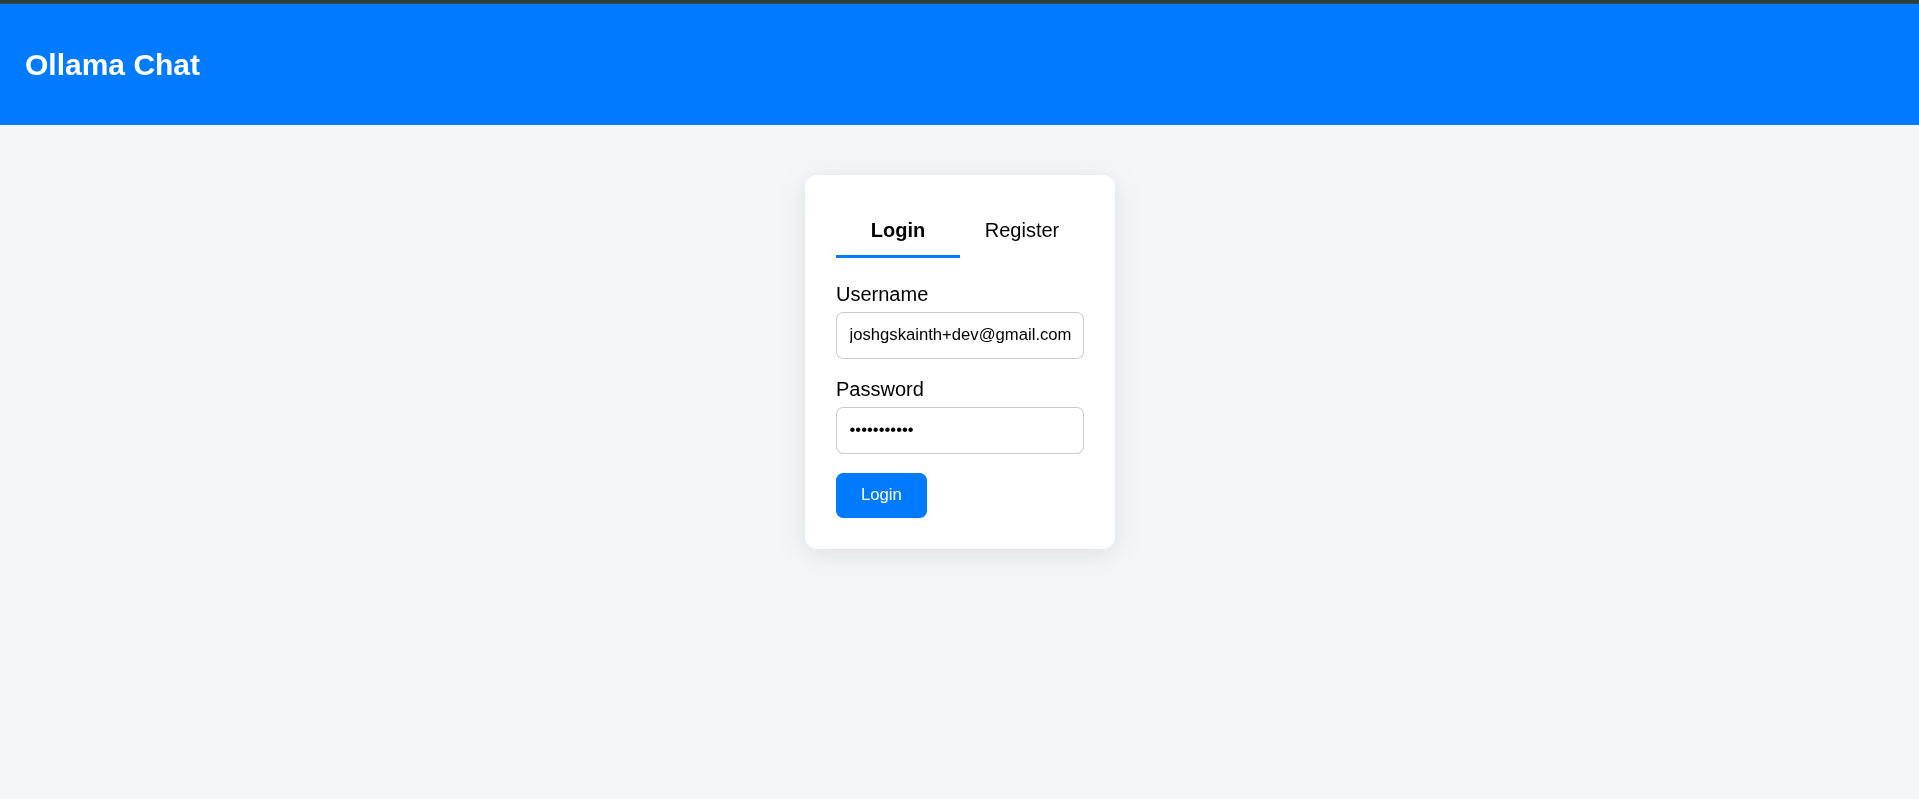
\includegraphics[width=0.9\textwidth]{assets/login_screen.png}
    \caption{Login and Registration Screen}
    \label{fig:login}
\end{figure}

\begin{figure}[H]
    \centering
    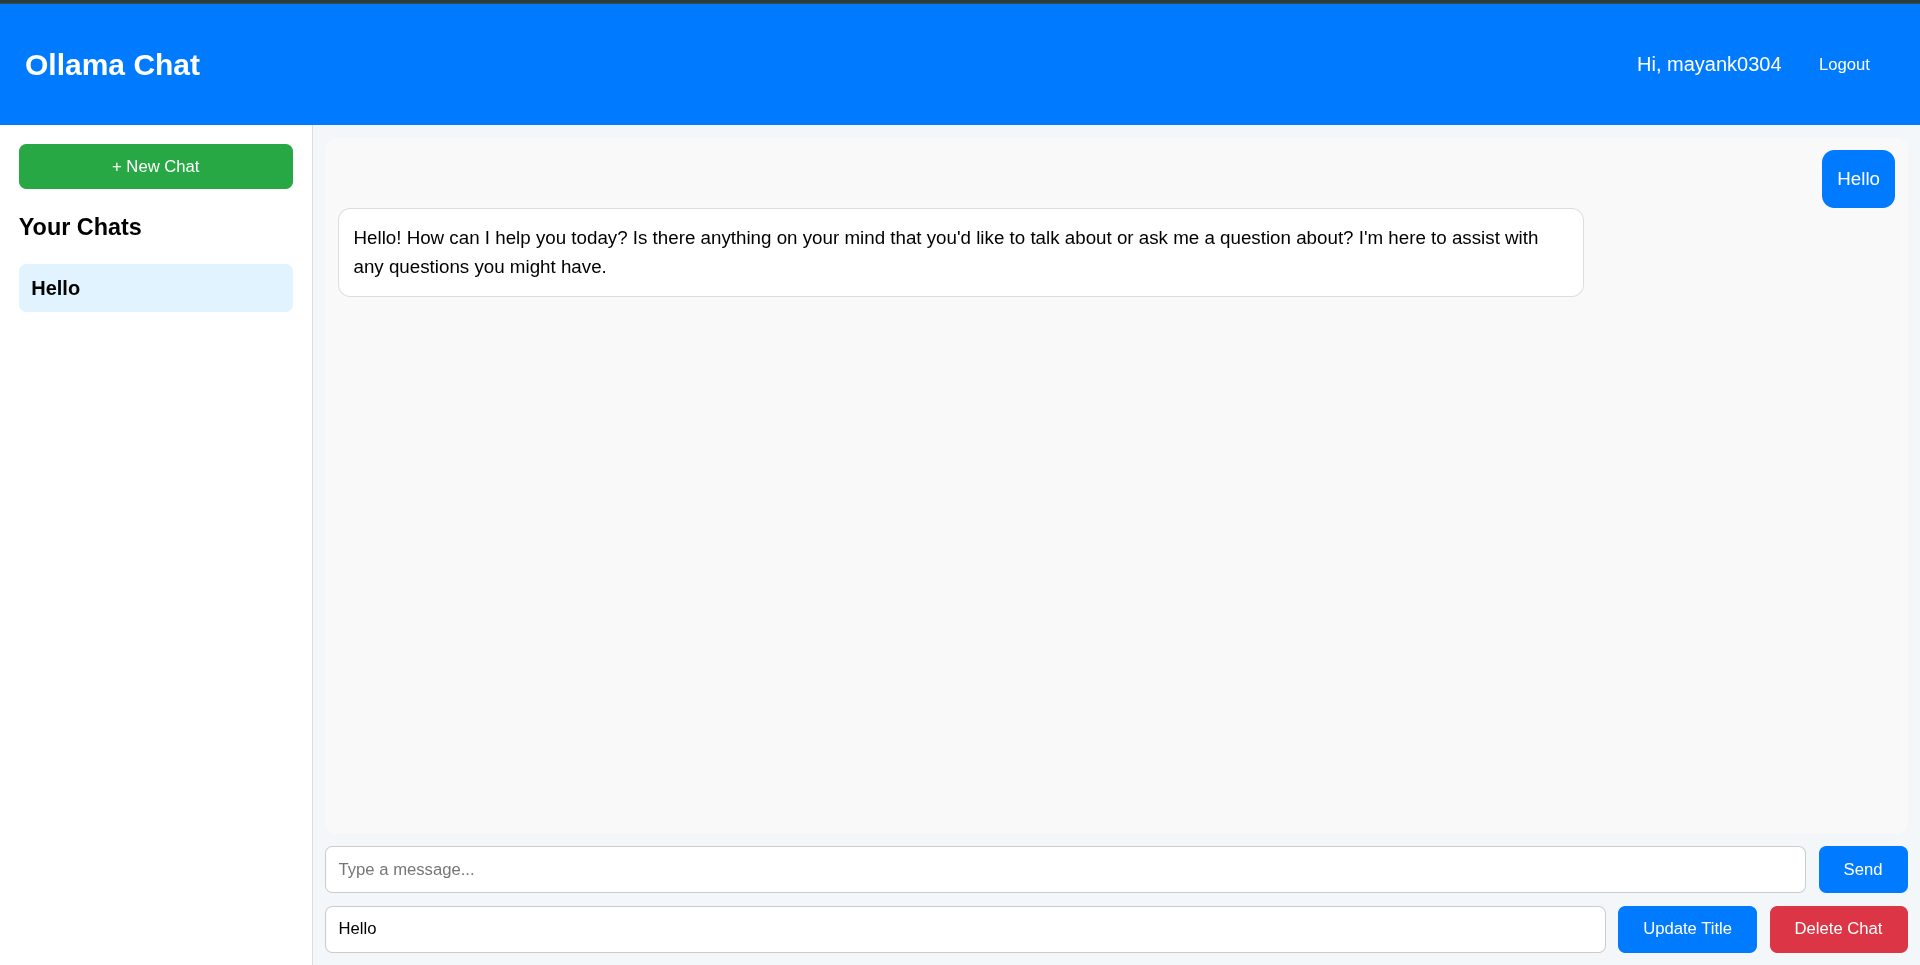
\includegraphics[width=0.9\textwidth]{assets/chat_interface.png}
    \caption{Main Chat Interface with Sidebar}
    \label{fig:chat}
\end{figure}

\section{Conclusion}
This project successfully demonstrates the implementation of a full-stack web application using the MEAN stack architecture. The integration of MongoDB provides a robust foundation for user authentication and chat history persistence, while Express.js delivers efficient API endpoints for both client-server communication and integration with the Ollama LLM service.

The application showcases several key aspects of modern web development:
\begin{itemize}
\item Effective use of NoSQL database design for flexible data storage
\item Implementation of secure authentication and session management
\item Creation of a responsive and intuitive user interface with AngularJS
\item Integration with external AI services through RESTful APIs
\item Complete CRUD operations for managing persistent user data
\end{itemize}

The project provides a solid foundation for further development and enhancement of AI-powered chat applications, demonstrating the capabilities of the MEAN stack in creating modern, interactive web experiences.

\end{document}
